% !TeX document-id = {489a4b48-3347-4d5e-985a-4bd4e83eb476}
% !TeX spellcheck = en_US
% !TeX encoding = UTF-8
% !TeX TXS-program:compile = txs:///latexmk/[-pdf -silent -shell-escape -latexoption="-synctex=1" -output-directory="build" -r "docstyle/nomenclature_latexmkrc"]
% !TeX TXS-program:quick = txs:///compile | txs:///view

\documentclass[english,sp]{docstyle/IDSCreport}

\title{Free Space Segmentation for Gokart Application}
\subtitle{V-Disparity}
\author{Noah Isaak}
\ethid{13-929-476}
\semester{FS 2019}
\email{nisaak@student.ethz.ch}
\supervision{First Supervisor\\ Prof. Dr. Second Supervisor}
\identification{IDSC-XX-YY-ZZ}
\date{December 2018}
\keywords{Ground detection, V-Disparity}
\bibliography{bibliography}

\begin{abstract}
Road and ground detection are closely related key tasks for an autonomous ground vehicle. These computations should be robust and preferably be performed in real-time. This paper aims to show the implementation of the V-Disparity method for ground detection. The approach is based on classic computer vision and does not incorporate learning methods. Basis of the method is a disparity map, for which a row-wise histogram is computed. This V-disparity histogram robustly preserves geometric scene features and can be used for various tasks. Experimental results however show the shortcomings of the implementation and how they could be overcome. In the following, a second pipeline is introduced. A mapping from a Velodyne Vld-16 Lidar to a camera is computed. The binary obstacle - ground mask which is computed from the lidar's point cloud can then be projected onto the camera image. These labels can then be used for e.g. machine learning tasks.


\end{abstract}

\begin{document}
% !TeX spellcheck = en_US
% !TeX encoding = UTF-8
% !TeX root = ../report.tex

\chapter{Introduction}
\label{chp:Introduction}

The tasks of segmenting a scene into ground, obstacles and other labels is a well-researched topic. It is a fundamental part of any autonomous ground vehicle, and lays the basis for many different tasks, such as planning, safety features or scene understanding. Over the last few years, solutions to this task, which are based on machine learning methods, have deemed themselves to be robust and accurate. Their ability to generalise and be applied to a variety of scenes make them a reliable choice. There however, exist many approaches to the problem, which are based on classic computer vision, with implementations dating few decades back. \newline
The goal of this semester project is the implementation of a robust and accurate free space detection pipeline based on classic computer vision. The results of this pipeline can be used to e.g. label data for machine learning. If the pipeline does not perform as expected, a second pipeline is introduced, where the focus entirely lies on labeling data for machine learning tasks. 

This semester project is part of a more extensive research into autonomous driving, based a self-driving Gokart. The Gokart is basis for a variety of research topics, such as planning, control systems and sensor fusion. The testing environment is a modular indoor Gokart track. The ground is flat, with no uphill or downhill sections. The track is not affected by weather conditions. 
\newline


\section{Related Work}
Related work on this topic is extensive. After limiting my research to the method of V-Disparity, early implementations can be dated back to 2002, with \cite{V-disparity_nonflat} providing a robust and accurate method for road detection, even for non-flat geometries. A study on the U-V Disparity method can be found in \cite{Hu2005}, providing a real-time implementation of the stereovision based scene analysis. The method was improved and adapted since it's introduction, becoming more robust and computationally efficient, as shown in \cite{Kakegawa2018}. Aside from free space detection, U-V-Disparity can be used solely for obstacle and pedestrian detection, with U-V-Disparity acting as the underlying basis for a SVM Classifier, where the extraced ROIs are used for training. Iloie et al. implemented this framework in \cite{Iloie2014}.
% !TeX spellcheck = en_US
% !TeX encoding = UTF-8
% !TeX root = ../report.tex

\chapter{Method}
\label{chp:Method}

\section{V-Disparity}

This chapter explains the theoretical basis of the V-disparity method. To begin with, the basis of the V-Disparity method, the disparity map, is outlined.

\subsection{Disparity Map} \label{sbs:method_dispmap}
It is assumed, that the reader has a general understanding of stereovision systems. Given two calibrated stereo cameras, the respective rectified images can be used to calibrate a disparity for each pixel. These is achieved with different block-matching algorithms, such as the StereoSGBM algorithm implemented in the popular OpenCV library. Given a disparity map, the baseline and focal length, a depth map can be calculated and used for further processing. The V-Disparity method however only makes use of the disparity map.


%Elaborate on calculation and formulas of disparity

\subsection{V-Disparity}

Once a disparity map $\Delta$(u,v) was computed, a V-Disparity histogram can be constructed. For each row u, a histogram of the occuring disparities in this row is computed. The histogram values represent the occurence of the respective disparity in the row, where each bin is represented by a pixel. Given a plane in a scene, the projection of the plane onto the V-Disparity image has a useful property. 
A plane will be projected as a linear curve in the V-Disparity image. This simplifies the extraction of the respective plane in the V-Disparity image, as a e.g. Hough Line Transform can be applied to detect the lines. Consequently, the detection of straight lines in the V-Disparity corresponds to detection of planes in the scene.
A scene is therefore made up of planes, where vertical planes can be understood as obstacles, horizontal planes as the road when flat, or as a set of oblique planes when the road is non-flat. Hu et al. \cite{Hu2005} offer an in-depth analysis of the projection of the three above types of planes.

\newline

Because the most prominent plane in usually represented by the ground, it will be detected as the line with the most votes in the V-Disparity image. Horizontal or vertical lines can be dismissed, as the disparity gradient of the road leads to a skewed line.
Horizontal lines can be associated with obstacles and used for obstacle detection.
Even though Non-flat road geometry will not be considered in this project, it should be noted that the road in that case can be approximated by a series of planes, which will then be projected as a piecewise linear curve in the V-Disparity image.

Once the line has been fitted in the V-Disparity image, the disparity values for the road surface are known. Extracting the road in the image domain is straightforward. For each row, the values which lie within a threshold of the value of the extracted line are part of the road, all other pixels are masked as non-road.

\begin{figure}
	\centering
	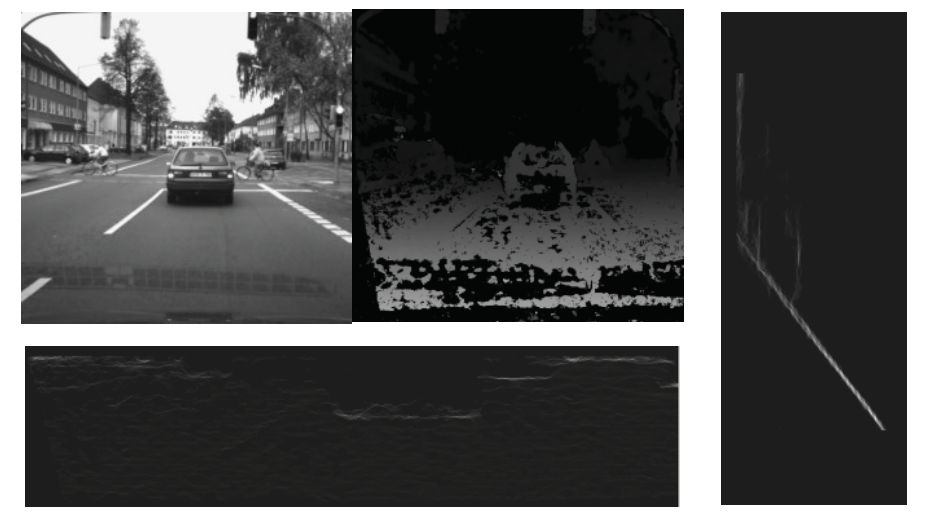
\includegraphics[width=0.7\linewidth]{Figures/vdisp}
	\caption[Overview of V-Disparity method]{}
	\label{fig:vdisp}
\end{figure}

Oniga et al. \cite{Oniga2015} show a camera image, the corresponding dispartiy map and the V- and U-Disparity respectively.



\section{Lidar Camera Projection}

To project lidar scanning points onto a camera image, the camera's intrinsic parameters should be known. Additionally, the projection matrix from lidar to camera should needs to be determined. It can be measured by hand and computed, or determined by externally calibrating the lidar and camera with an automated pipeline.
\newline
After driving a few laps on our indoor Gokart track, the lidar generates an occupancy grid. This occupancy grid is then projected onto the camera frame. By determining the relative pose and orientation of the camera with respect to the world frame, one can then project all points corresponding to the road onto the camera frame.
% !TeX spellcheck = en_US
% !TeX encoding = UTF-8
% !TeX root = ../report.tex

\chapter{Implementation}
\label{chp:Implementation}


\section{V-Disparity Implementation}
\label{vdisp_impl}


\section{Hardware}

The Gokart is fitted with a ZED Stereolabs camera, see Figure \ref{fig:zedproductmain}, which was the basis for the V-Disparity method. The camera comes with a ZED SDK, which provides many functionalities, such as disparity map generation and point cloud computation. The Python API enables quick and intuitive access to these functionalities.
In addition, a Velodyne VLD-16 Lidar is mounted on top of the Gokart, which can be seen in Figure \ref{fig:lidar}. It offers 16 scanning lines with high accuracy.
More infos on the used hardware can be found on the manufacturer's website.

\begin{figure}
	\centering
	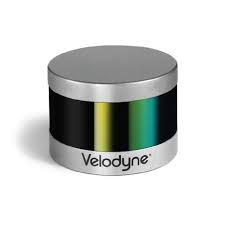
\includegraphics[width=0.5\linewidth]{Figures/lidar}
	\caption[Velodyne Vld-16 Lidar Sensor]{}
	\label{fig:lidar}
\end{figure}

\begin{figure}
	\centering
	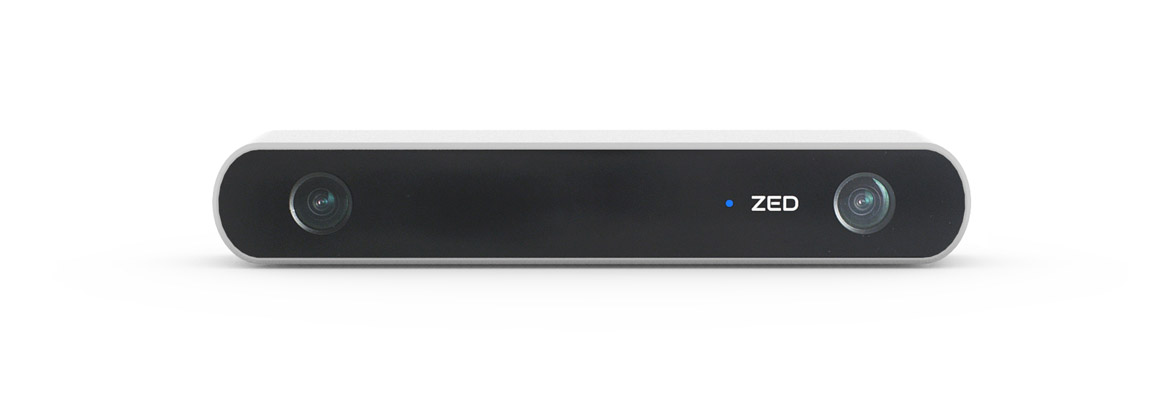
\includegraphics[width=0.7\linewidth]{Figures/ZED_product_main}
	\caption[ZED Stereolabs Camera]{}
	\label{fig:zedproductmain}
\end{figure}



\section{Code implementation}

The method was implemented in the Python framework, while making use of the popular OpenCV library. OpenCV was used, mainly because of the existing methods already implemented, such as the probabilistic houghline transform, which was used for line-fitting. The OpenCV aims at real-time computer vision programming functions, which is a crucial property for autonomous vehicles.
\newline

Given the ZED Camera and the ZED SDK, data can be streamed from the Camera with few lines of code. Depending on the application, the resolution, framerate and other parameters can be adjusted accordingly. For disparity computation, range and quality can be modified, to fit the requirements.
The disparity map is computed as float32. For visualisation purposes, a normalisation and conversion to uint8 type needs to be done. 
For higher precision, the float32 disparity map can be used for further processing. 
To ease up on computation, the uint8 disparity map was used for the V-Disparity method. The number of histogram bins for every row histogram is then set to 255, one for every disparity value present in the normalised disparity image. OpenCV's calcHist function was used.
To extract the regions of interest, in our case the ground, OpenCV's Houghline transform can be used, to fit the line in the image. In order to fine tune the line fitting, probabilistic houghline transform was used, where minimum line length and maximum line gap can be adjusted. This line can then be backprojected into the original camera image, to generate the mask.

For the current implementation, the disparity map and camera images are streamed at a resolution of (672, 376). The same resolution is used for the V-Disparity Histogram and Line Fitting. For mask generation, the resolution was downscaled by a factor of two, to ease up on computation and enable real-time application. Using higher resolution could improve results, but drastically lowers the framerate

%insert figure of pipeline, from stereo image to disparity image to v-disparity image and fitted line, and finally the resulting mask.


In order to avoid speckles and disjointed mask segments, all mask pixels are labeled according to their connectedness, using OpenCV's connectedComponents function. Only the largest connected region is kept, all other labels are discarded. 
% !TeX spellcheck = en_US
% !TeX encoding = UTF-8
% !TeX root = ../report.tex

\chapter{Results}
\label{chp:Results}

Results have been visually evaluated, as there is no ground truth available for this method. 
The evaluation have shown, that for this project's implementation, the V-Disparity method does not provide the desired results. The generated mask lacks temporal coherency, and for mid-range distances (>4m), important features are not detected, such as various obstacles or road boundaries. 
\newline
The reason for this can be found in the generated disparity map. Without post processing, the backprojection of the road requires an accurate disparity map. However the quality of the disparity map diminishes for further distances, edges are not well preserved and artifacts in low-textured areas lead to inaccurate masks.
\newline

% !TeX spellcheck = en_US
% !TeX encoding = UTF-8
% !TeX root = ../report.tex

\chapter{Conclusion}
\label{chp:Conclusion}

The evaluation of the proposed V-Disparity method for free-space detection shows the need for an auxiliary sensor, in our case a range finding lidar sensor. The stereocamera on it's own does not provide the desired quality of the road mask. To complete the task of creating a useful road mask, a second method was implemented, which projects scanned lidar points into the camera frame. This was done by first externally calibrating the two sensors, after meticulously measuring the relative pose and orientation. This approach was then compared to a automatic calibration method, which is available online.

\subsection{Future Work}
For future work, the disparity map generation should be improved. The quality of disparity maps generated by recent neural networks seem promising, such as PSMNet by Jlia et al.  \cite{DBLP:journals/corr/abs-1803-08669}. Resolving the bottleneck of the disparity map can shed light on the performance of the actual V-Disparity method. Keeping the initial ground mask undersegmented, and refining it by using it as seeds for region growing algorithms, may improve results.
Augmenting the code to be more computationally efficient should be considered as well. Using for loops in Python increases computing time, replacing loops with other functionalities can help.

\appendix
% !TeX spellcheck = en_US
% !TeX encoding = UTF-8
% !TeX root = ../report.tex

\chapter{Example Appendix Chapter}
\label{chp:ExampleAppendixChapter}

The following code is the definition of the bibliography entry of the document class IDSCreport~\cite{IDSCreportClass}.

\lstinputlisting[style=plaincode,xleftmargin=1em]{bibliography.bib}
\end{document}
